\documentclass{beamer}
\usepackage[utf8]{inputenc}
\usepackage[authoryear]{natbib}
\usepackage{subfigure}
\usepackage[noend]{algpseudocode}
\usepackage{color}
\usepackage{alltt}
\usepackage{tabularx}
\usepackage{amsmath,amssymb}
\usepackage{microtype}
\usepackage{tikz}
\usetikzlibrary{fit,positioning}

\setbeamertemplate{navigation symbols}{} 

\usepackage{multimedia}

%\usetheme{none}
%\usecolortheme{albatross}

\newenvironment{centercolumns}{\begin{columns}[c]}{\end{columns}}
%\newcommand{\newblock}{}


\newcommand{\dataset}{\mathcal{D}}
\newcommand{\model}{\mathcal{M}}
\newcommand{\parameters}{\theta}
\newcommand{\vparameters}{\phi}
\newcommand{\vy}{\mathbf{y}}
\newcommand{\vx}{\mathbf{x}}
\newcommand{\diff}{\mathrm{d}}

\title{Probabilistic inference for big data}
\author{Arto Klami and Antti Honkela}
\date{6 March 2015}



\begin{document}

\frame{\titlepage}

%\frame{\frametitle{Outline} \tableofcontents}

\section{Introduction}

\begin{frame}
  \frametitle{Statistical machine learning}

  \begin{itemize}
  \item Machine learning: Interest in general models, tools applicable
    for various kinds of data
  \item Robustness and scalability often important
  \item Here we talk about models based on Bayesian inference
  \end{itemize}
\end{frame}

\begin{frame}
  \frametitle{Bayesian inference}

  \begin{itemize}
  \item Given a model family ${\cal M}$ and some data $D$, estimate
    the posterior distribution $p(\theta|D,{\cal M})$ of the model
    parameters
  \item Often used for predictions by averaging over the posterior
  \item Bayes rule:
    \[
    p(\theta|D) = \frac{p(D|\theta)p(\theta)}{p(D)}
    \]
  \end{itemize}
\end{frame}

\begin{frame}
  \frametitle{Latent variable models}

  Models with
  \begin{itemize}
  \item Small(ish) set of \emph{global} parameters
  \item Large set of \emph{latent variables} or \emph{local} parameters
  \end{itemize}

  Examples:
  \begin{itemize}
  \item Gaussian mixture model: Global parameters are the means,
    variances and prior weights, local parameters are the sample
    allocations
  \item Topic model: Global parameters are topic-to-word distributions,
    local parameters are the document-to-topic distributions
  \end{itemize}
\end{frame}

\begin{frame}
  \frametitle{Big data}

  \begin{itemize}
  \item Oxford English Dictionary: ``data of a very large size, typically to the extent that its manipulation and management present significant logistical challenges''
  \item Wikipedia: ``any collection of data sets so large and complex that it becomes difficult to process using on-hand data management tools or traditional data processing applications''
  \item Tom Davenport: ``The broad range of new and massive data types that have appeared over the last decade or so.''
  \item Corporate meaning: ``Any data not in our SQL'' (this we would just call data)
  \end{itemize}

  \begin{itemize}
  \item Sometimes we simply have a lot of data, which means we
    have to pay attention to computation speed as well, without losing
    rigor
  \end{itemize}
\end{frame}

\begin{frame}
  \frametitle{Big data}

  \begin{itemize}
    \item Next generation sequencing: Terabytes of data per day
    \item Brain imaging: fMRI scanner produces around $10^8-10^9$
      measurements per hour
    \item Twitter: 500 million per day, one-second peak record 140k
  \end{itemize}

\end{frame}

\begin{frame}
  \frametitle{Bayesian inference for big data}

  Imagine running a MCMC sampler to infer sentiment of the tweets
  in real time... Fast distributed hardware is not going to be enough.

  \begin{itemize}
  \item Evaluating the Bayes rule has $\mathcal{O}(n)$ complexity
    for $n$ samples (even for the simplest models that assume independence)
  \item What if $n$ is one billion? One trillion? We need to get below
    linear complexity
  \item Intuitively: data as a resource, we do not need to
    use it all if less is enough to solve the problem
  \item For latent variable models, the problem is optimizing the
    global parameters without knowing all of the local ones
  \end{itemize}
\end{frame}

\begin{frame}
  \frametitle{Approaches}

  \begin{itemize}
    \item Variational inference: Optimization for Bayesian inference
    \item Scalable variational inference
    \item Scalable MCMC
  \end{itemize}
\end{frame}

\section{VB}

% TODO: Split basic into 2-3 slides, bring in an example

\begin{frame}
  \frametitle{Variational inference basics}

  \begin{itemize}
  \item Idea: approximate the posterior distribution $p(\parameters | \dataset)$
    with another distribution $q(\parameters)$ that is analytically tractable
  \item Learn the approximation by minimizing the distance between $q(\parameters)$ and $p(\parameters | \dataset)$
  \item The distance is measured by the Kullback-Leibler divergence
    $D(q||p) = \int q(\parameters) \log \frac{q(\parameters)}{p(\parameters| \dataset)}\diff \parameters$
  \item ...and the minimization is often converted into maximizing a lower bound on the marginal
    likelihood (ELBO):
    $L = \int q(\parameters) \log \frac{p(\dataset,\parameters)}{q(\parameters)} \diff \parameters= p(\dataset) - D(q||p)$
  \item Predictions then made by replacing $\int p(\vx|\parameters) p(\parameters | \dataset) \diff \parameters$ by
    $\int p(\vx|\parameters) q(\parameters) \diff \parameters$
  \end{itemize}
\end{frame}

% TODO: Present this already in the gradient form, just
% concluding that we actually get closed-form updates

\begin{frame}
  \frametitle{Mean-field variational inference}

  \begin{itemize}
    \item Often $q(\parameters)$ is factorized as $\prod_i q(\parameters_i)$, so that
      we can optimize one factor at a time
    \item Differentiating wrt to $q(\parameters_i)$ and setting the derivative to zero provides a closed-form
      update $\log q(\parameters_i) = \int q(\parameters_{-i}) \log p(\dataset, \parameters) \diff \parameters_{-i} + C$
    \item The expectation over all other factors is typically easy to compute fo
r exponential
      family distributions with conjugate priors (and much harder for everything else)
    \item Leads to an algorithm closely resembling expectation maximization
  \end{itemize}
\end{frame}

% TODO: Introduce stochastic optimization properly; Robbis-Monro etc

\begin{frame}
  \frametitle{Towards more scalable variational inference}

  \begin{itemize}
  \item Given a parametric form $q(\parameters|\vparameters)$ VB is an optimization problem:
  $L(\vparameters) = \int q(\parameters|\vparameters) \log \frac{p(\dataset,\parameters)}{q(\parameters|\vparameters)} \diff \parameters$
  \item Gradient-based optimization generally applicable: $\vparameters \leftarrow \vparameters + \delta
    \nabla L(\vparameters)$
  \item Natural gradient speeds up convergence: Replace $\nabla L(\vparameters)$ with $F^{-1}(\vparameters)
\nabla L(\vparameters)$, where $F(\vparameters)$ is the Fisher information matrix
  consisting of expectations of second derivatives of $\log q(\parameters | \vparameters)$
 (Honkela et al., JMLR 2010)
  %\item Stochastic gradients applicable (Hoffman et al., JMLR 2013); more about this during the seminar
  \end{itemize}
\end{frame}

\begin{frame}
  \frametitle{Variational inference example}

  \begin{figure}
  \begin{center}
  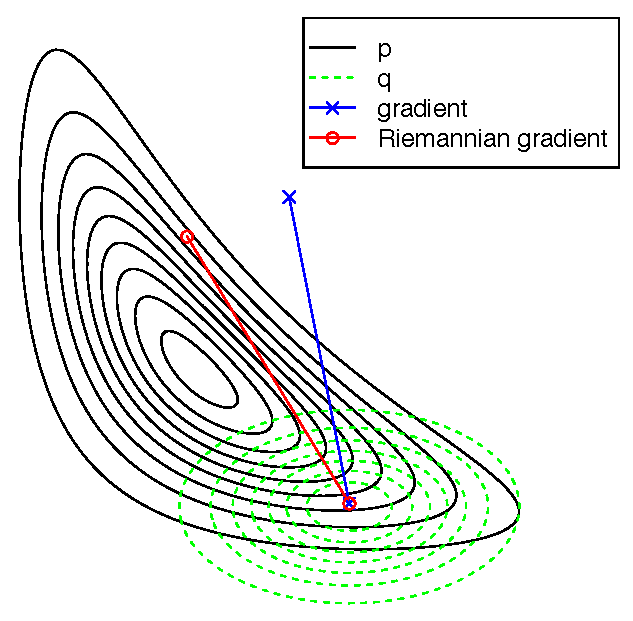
\includegraphics[width=0.7\textwidth]{VBnatgrad.pdf}
  \end{center}
  \end{figure}
  \vfill \hfill {\tiny Figure from Honkela et al. (JMLR 2010)}
\end{frame}

\begin{frame}
  \frametitle{Stochastic variational inference}

  \begin{enumerate}
  \item M.D. Hoffman, D.M. Blei, C. Wang, J. Paisley. \textbf{Stochastic Variational Inference}, JMLR 2013
  \end{enumerate}

  \begin{itemize}
    \item Well-written description of the above ideas
    \item TODO: Pick the algorithm from the paper
  \end{itemize}
\end{frame}

\begin{frame}
  \frametitle{Stochastic optimization -- how exactly?}

  \begin{enumerate}
    \item Extensive literature on stochastic optimization
    \item Adagrad, Nesterov, smoothing/memory etc for choosing the step lengths
      and directions automatically (TODO: Mention some papers)
    \item Active research topic, illustrating a nice merger of
      previously separate communities
  \end{enumerate}
\end{frame}

\begin{frame}
  \frametitle{Some more elaborate examples}

  \begin{enumerate}
  \item J. Hensman, N. Fusi, N.D. Lawrence, \textbf{Gaussian Processes for Big Data}, UAI 2013.
  \item J. M. Hernandez-Lobato, N. Houlsby, Z. Ghahramani, \textbf{Stochastic Inference for Scalable Probabilistic Modeling of Binary Matrices}, ICML 2014.
  \end{enumerate}

%  \begin{itemize}
%  \item GP inference
%    $$ y_i = f(\vx_i) + \epsilon $$
%  \item Variational sparse GPs: introduce \emph{inducing variables}
%    $$ \mathbf{u} = [f(\mathbf{z}_i)]_{i=1}^m $$
%  \item Standard variational GPs collapse $\mathbf{u}$, but that
%    cannot be done with SVI
%  \end{itemize}

%  \begin{itemize}
%  \item Subsample both data points and ``global variables''
%  \item Nice method for deciding mini-batch size
%  \end{itemize}
\end{frame}

%\section{Other}

%\begin{frame}
  % Arto + Antti
%  \frametitle{Stochastic gradients in general}

%  \begin{enumerate}
%  \item M. Schmidt, N. Le Roux, F. Bach, \textbf{Minimizing Finite Sums with the Stochastic Average Gradient}, arXiv 2013.
%  \end{enumerate}
%  \begin{itemize}
%  \item Basic idea: introduce a memory of gradients and simply update the
%    component from one data point or mini-batch at a time
%  \item Improves the asymptotic convergence rate
%  \end{itemize}

%\end{frame}


\section{MCMC}

% Antti

\begin{frame}
  % Antti
  \frametitle{Approximate inference by sampling}

  \begin{itemize}
  \item A lot of Bayesian inference boils down to computing integrals
    $$ E[f(\parameters)] = \int_\parameters f(\parameters) p(\parameters | \dataset) \diff\parameters $$
    \begin{itemize}
    \item Model predictions, posterior statistics of parameters, \dots
    \end{itemize}
  \item $\parameters$ is often high-dimensional which makes these very difficult
  \item Stochastic approximation:
    $$ E[f(\parameters)] \approx \frac{1}{N} \sum_{i=1}^N f(\parameters_i), $$
    when $\parameters_i \sim p(\parameters | \dataset)$
  \item How to simulate samples following a given distribution?
  \end{itemize}
\end{frame}

\begin{frame}
  \frametitle{MCMC basics (Metropolis et al., 1953; Hastings, 1970)}

  \begin{itemize}
  \item Idea: construct a Markov chain, whose stationary distribution
    is the distribution of interest $p(\parameters | \dataset)$
  \item Requires an \emph{unnormalised} $p^*(\parameters | \dataset) \propto
    p(\parameters | \dataset)$
  \item In the Bayesian setting typically
    $$ p(\parameters | \dataset) = \frac{p(\dataset | \parameters) p(\parameters)}{p(\dataset)} $$
    which easily yields the unnormalised density
    $$ p^*(\parameters | \dataset) = p(\dataset | \parameters) p(\parameters) $$
  \item To define the Markov chain, we need to specify a transition
    distribution $q(\parameters' | \parameters)$
  \item The Markov chain is guaranteed to converge if it satisfies
    sufficient regularity conditions and the \emph{detailed balance}
    condition
    $$ q(\parameters' | \parameters) p(\parameters | \dataset) =
       q(\parameters | \parameters') p(\parameters' | \dataset) $$
  \end{itemize}
\end{frame}

\begin{frame}
  \frametitle{Metropolis--Hastings algorithm}

  \begin{itemize}
  \item The most widely used MCMC algorithm is the Metropolis--Hastings
    algorithm
  \item Accept--reject mechanism, proposals are accepted with probability
    $$ f(\parameters' | \parameters) = \min\left(1, \frac{\color{blue}q(\parameters | \parameters') p(\parameters' | \dataset)}
      {\color{red}q(\parameters' | \parameters) p(\parameters | \dataset)} \right) $$
  \item This satisfies the detailed balance because
    \begin{align*}
      {\color{red}f(\parameters' | \parameters)
      q(\parameters' | \parameters) p(\parameters | \dataset)}
      &= \min({\color{blue}q(\parameters' | \parameters) p(\parameters | \dataset)},
      {\color{red}q(\parameters | \parameters') p(\parameters' | \dataset)}) \\
      &= \min({\color{red}q(\parameters | \parameters') p(\parameters' | \dataset)},
      {\color{blue}q(\parameters' | \parameters) p(\parameters | \dataset)}) \\
      &= {\color{blue}f(\parameters | \parameters')
      q(\parameters | \parameters') p(\parameters' | \dataset)}
    \end{align*}
  \end{itemize}
\end{frame}

\begin{frame}
  \frametitle{MCMC for big data}

  \begin{itemize}
  \item The challenge for big data: likelihood computation needed for
    acceptance decision needs all data
  \item Proposed solutions
    \begin{enumerate}
    \item Work on subsets of data
    \item Approximate the acceptance decision
    \item Make better proposals that avoid acceptance checks
    \end{enumerate}
  \end{itemize}
\end{frame}

\begin{frame}
  \frametitle{Solution 1: Subset and parallelised sampling}

  \begin{itemize}
  \item W. Neiswanger, E. Xing, C. Wang, \textbf{Asymptotically Exact, Embarrassingly Parallel MCMC}, UAI 2014
  \end{itemize}

  \begin{itemize}
  \item Factorise the posterior
    $$ p(\parameters | \dataset) \propto \prod_{m=1}^M \left[ p(\parameters)^{\frac{1}{M}} p(\dataset_m | \parameters) \right], $$
    where $\dataset = \bigcup_{m=1}^M \dataset_m$
  \item Sample from each subposterior independently in parallel
  \item Combine the samples using density estimates
  \end{itemize}
\end{frame}

\begin{frame}
  \frametitle{Solution 2: Approximate acceptance}

  \begin{itemize}
  \item A. Korattikara, Y. Chen, M. Welling, \textbf{Austerity in MCMC Land: Cutting the Metropolis--Hastings Budget}, ICML 2014.
  \end{itemize}

  \begin{itemize}
  \item Basic idea: more efficient use of data by approximating the
    Metropolis--Hastings accept/reject choice
  \end{itemize}
\end{frame}

\begin{frame}
  % Antti
  \frametitle{Solution 3: Better proposals using gradients}
  % HMC etc

  \begin{itemize}
  \item Standard MCMC is based on proposal distributions whose shape is
    essentially \emph{independent of the target}
    \begin{itemize}
    \item E.g.~fixed multivariate Gaussian proposals
    \end{itemize}
  \item Target distribution gradients would allow utilising local shape
  \item Common algorithms:
    \begin{itemize}
    \item Langevin dynamics MCMC
    \item Hamiltonian Monte Carlo  (a.k.a. hybrid Monte Carlo)
    \end{itemize}
  \item Both based on constructing a suitable dynamical system and
    simulating it
  \end{itemize}
\end{frame}

\begin{frame}
  \frametitle{Langevin and Hamiltonian dynamics in MCMC}

  Langevin dynamics proposal:
  $$ \parameters^* = \parameters + \frac{\epsilon}{2} \nabla_\parameters \log p(\dataset, \parameters) + N(0, \epsilon I) $$
  \begin{itemize}
  \item Acceptance rate tends to one as $\epsilon \rightarrow 0$
  \end{itemize}
  \mbox{}\\
  Hamiltonian MCMC:
  \begin{itemize}
  \item Construct a Hamiltonian dynamical system with momentum
  \item Hamiltonian ($\approx$ ``energy'') is conserved in simulation
  \item Can take arbitrarily long steps, assuming the Hamiltonian
    system can be simulated accurately
    \begin{itemize}
    \item Symplectic geometry studies this problem
    \end{itemize}
  \end{itemize}
\end{frame}

\begin{frame}[allowframebreaks]
  % Arto + Antti
  \frametitle{Stochastic gradients with MCMC}

  \begin{itemize}
  \item M. Welling, Y.W.Teh, \textbf{Bayesian Learning via Stochastic Gradient Langevin Dynamics}, ICML 2011 and S. Ahn, A. Korattikara, M. Welling, \textbf{Bayesian posterior sampling via stochastic gradient Fisher scoring}, ICML 2012.
  \item T. Chen, E. Fox, C. Guestrin, \textbf{Stochastic Gradient Hamiltonian Monte Carlo}, ICML 2014.
  \end{itemize}

  \begin{itemize}
  \item Stochastic gradient proposal, always accept
  \item Convergence theory needs step sizes shrinking to zero, often
    ignored in practice
  \end{itemize}
\end{frame}


\begin{frame}
  \frametitle{Summary}

  \begin{itemize}
  \item VB algorithms rest on solid theoretical foundation with SGD
  \item Ensuring convergence in practice can still be tricky
  \item Big data MCMC theoretical analysis still developing
  \item Cautionary tales from skipping MH-step
  \item Subset and austerity approaches seem more reliable, but may
    still have gotchas
  \end{itemize}
\end{frame}


\end{document}
